\chapter{Architecture Diagram and Conceptual Model}

\section{Architecture}
The system relies on an event-based architecture. As shown in the architecture diagram (Figure \ref{fig:architecture}), the arrows show the flow of data between the different components of the system. The doorbell button triggers an event that goes to the Raspberry Pi Zero which acts as an announcer in this architecture. This event tells the announcer to broadcast the appropriate doorbell event to all types of devices currently registered in the system. The doorbell offers feedback to the Visitor in the form of a pulsating light to confirm that the button was pressed and the event was broadcast to the Resident's devices. The arrow going to the Raspberry Pi Zero from the Home Network is to confirm that the devices received the broadcast event.

The architecture is event-driven. Each of the parts are in a waiting state. Once a trigger is sent, the state will change to its respective action and then repeat to a waiting state. The entire system is triggered solely by the Doorbell. It, being in a low-power waiting state, will wake up on a doorbell press and alert the Raspberry Pi Zero. The Raspberry Pi Zero will then have to process the package, alerting the respective devices through the Wi-Fi router. The Philips Hue Lights and other devices in the system will leave their waiting states once alerted through the Wi-Fi router and begin to notify the resident. All states are reverted back to waiting once the devices have finished notifying the resident. The advantage of having all devices to maintain a waiting state is that we can more quickly notify the user. The disadvantage is that the system will require more power. Fortunately, the only part of our system that would require that is the doorbell which would generally be outside, unable to plug into an outlet. The Raspberry Pi Zero can be plugged into an outlet. The best option would be to connect it next to the router and use an Ethernet cable to connect to the Wi-Fi router. The Philips Hue lights and other devices will be per-user requirement. Certain devices may operate on battery but that is not a concern of this project, but rather a concern for the resident.

\begin{figure}[ht]
  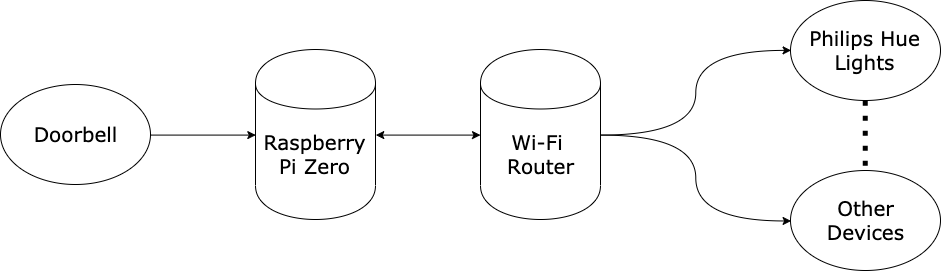
\includegraphics[width=0.9\textwidth]{Architecture-updated.png}
  \centering
  \caption{Architecture Diagram}
  \label{fig:architecture}
\end{figure}

\section{Conceptual Model}
The system uses the Raspberry Pi Zero as the main gateway. A router will be necessary in communicating to other devices in the household. The button of the doorbell will be attached to the an Arduino and communicate with the Raspberry Pi Zero. Since Arduino and Raspberry Pi do not come with 802.15.4 capabilities, an XBee was used to communicate between the devices. Furthermore, to abstract user experience, a smartphone application would be necessary to control the system. With simple actions, the resident should be able to perform all Use-Case actions described in Chapter 3. The system also uses a variety of communication protocols, so the appropriate hardware modules will be necessary.

\begin{figure}[ht]
  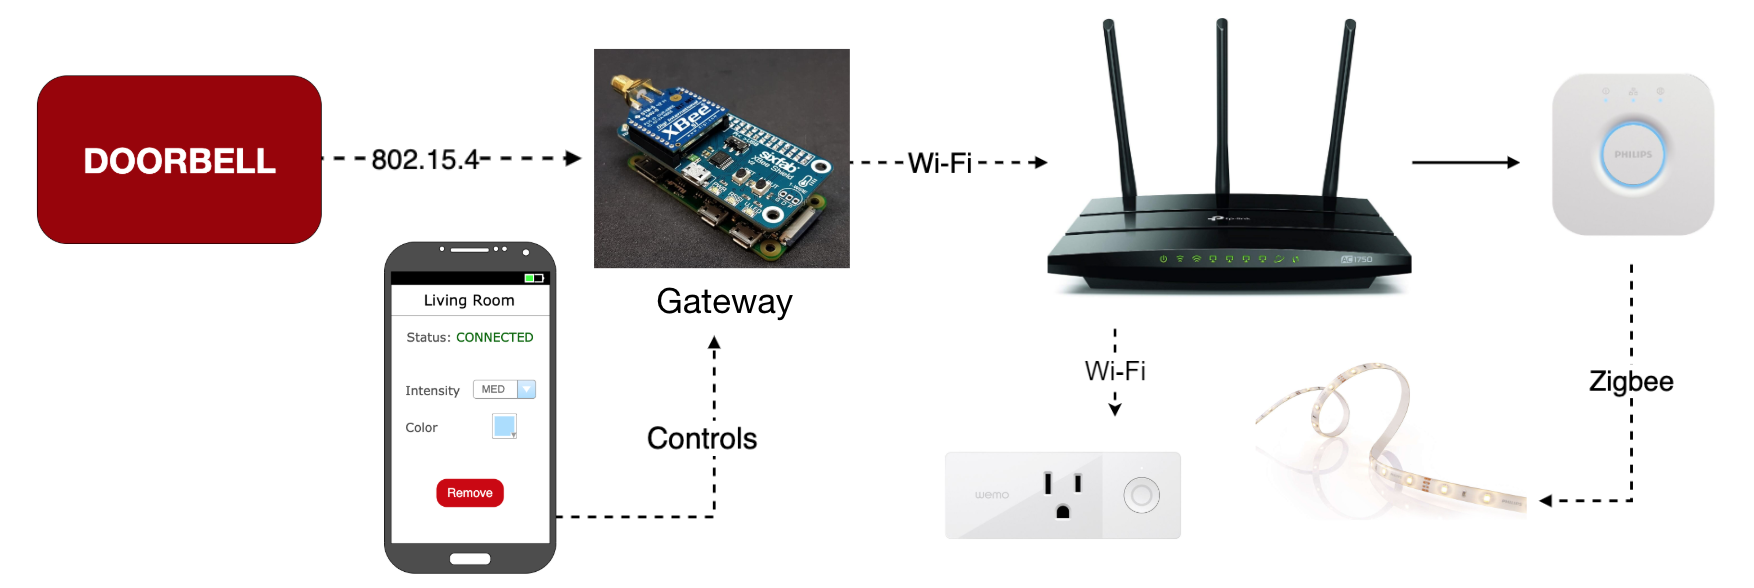
\includegraphics[width=0.8\textwidth]{senior-design-model.png}
  \centering
  \caption{Conceptual Model}
  \label{fig:conceptualmodel}
\end{figure}